\documentclass{standalone}
\usepackage{tikz}
\usepackage{ctex,siunitx}
\setCJKmainfont{Noto Serif CJK SC}
\usepackage{tkz-euclide}
\usepackage{amsmath}
\usetikzlibrary{patterns, calc,3d}
\usetikzlibrary {decorations.pathmorphing,decorations.pathreplacing,decorations.shapes}
\begin{document}
\small
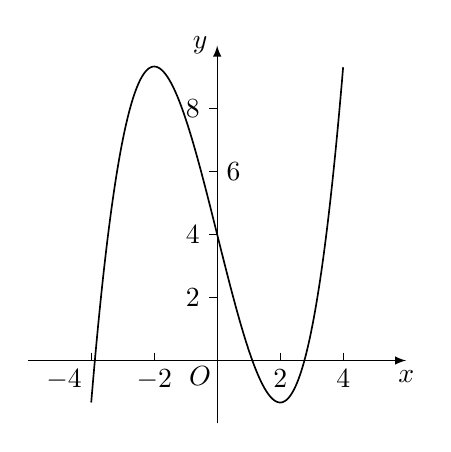
\begin{tikzpicture}[>=latex,scale=0.4]
  \draw[->](-6,0)--(6,0)node[below]{$x$};
  \draw[->](0,-2)--(0,10)node[left]{$y$};
  \draw[semithick,samples=200,domain=-4.0:4.0]plot(\x,4-4*\x+1/3*\x*\x*\x);
  \foreach \x in {-2,2,4}
  {
    \draw[very thin](\x,0.25)--(\x,0)node[below]{$\x$};
  }
  \draw[very thin](-4,0.25)--(-4,0)node[below left]{$-4$};
  \foreach \x in {2,4,8}
  {
    \draw[very thin](0,\x)--(-0.25,\x)node[left]{$\x$};
  }
  \draw[very thin](0,6)--(-0.25,6)node[at start,right]{$6$};
  \node at (0,0)[below left,inner sep=2pt]{$O$};
\end{tikzpicture}
\end{document}